% ============================================================
%  sec-2-training-lifecycle.tex  —  3.2 Training Lifecycle
% ============================================================

\section{Complete Nemotron Training Lifecycle}
\label{sec:training-lifecycle}

The Nemotron 3 Nano training pipeline is structured as a sequential
three-stage process documented across four directories in the repository:
\filepath{stage0\_pretrain/}, \filepath{stage1\_sft/}, \filepath{stage2\_rl/},
and \filepath{stage3\_eval/}. Each stage consumes the checkpoint artifact
produced by the previous stage, forming a lineage chain tracked through
Weights \& Biases artifacts. The complete pipeline flow is illustrated
in \figref{pipeline-overview}.

% ── Figure 3.2 placeholder ───────────────────────────────────
\begin{figure}[H]
    \centering
    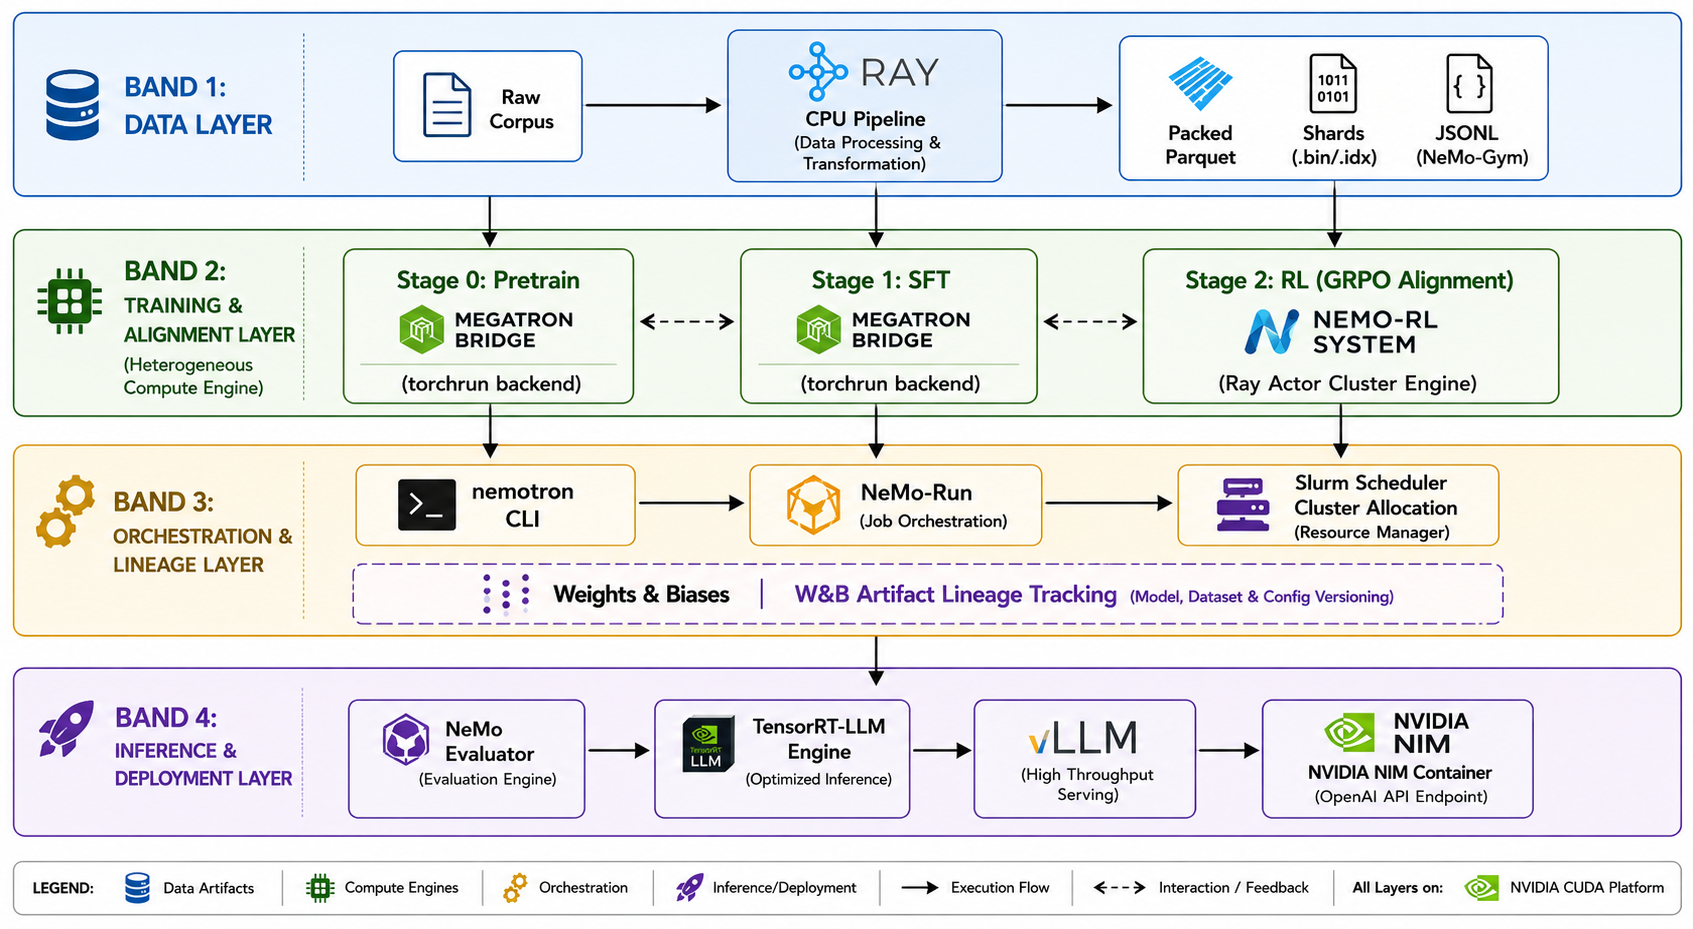
\includegraphics[width=0.85\textwidth]{images/figures/end2endnemopipeline.png}
    \caption{End-to-End Nemotron AI training pipeline Overview}
    \label{fig:pipeline-overview}
\end{figure}

% ── 3.2.1 ────────────────────────────────────────────────────
\subsection{Data Preparation}
\label{subsec:data-prep}

\subsubsection{Pretraining Data Preparation}
\label{subsubsec:pretrain-data-prep}

The pretraining data pipeline is implemented in
\filepath{stage0\_pretrain/data\_prep.py}. Its purpose is to tokenize raw
text corpora into Megatron's binary format (\texttt{.bin}/\texttt{.idx})
required by Megatron-Bridge's data loader.

The pipeline executes three sequential stages managed by the
\texttt{cosmos\_xenna.pipelines.v1} framework:

\begin{enumerate}
  \item \textbf{PlanStage}: Reads the dataset blend definition from
        \filepath{config/data\_prep/data\_blend\_raw.json}, performs
        deterministic work-item hashing, and generates per-shard
        \texttt{DatasetWorkItem} objects.
  \item \textbf{DownloadStage}: Fetches each dataset shard from its
        source (Hugging Face Hub or local storage), one node per shard.
  \item \textbf{BinIdxTokenizationStage}: Tokenizes documents using the
         tokenizer
        (\texttt{add\_bos=False}, \texttt{add\_eos=True}) and writes
        \texttt{.bin}/\texttt{.idx} file pairs.
\end{enumerate}

\begin{table}[htbp]
  \centering
  \caption{Pretraining data preparation: inputs, outputs, and configuration}
  \label{tab:pretrain-data-prep}
  \begin{tabularx}{\textwidth}{>{\hsize=0.6\hsize}L >{\hsize=1.4\hsize}L}
    \toprule
    \tableheader{Property & Detail} \\
    \midrule
    Entry point    & \texttt{stage0\_pretrain/data\_prep.py} \\
    \rowcolor{TableRowOdd}
    Input format   & Raw text datasets (HF Hub or local); blend defined in
                     \texttt{config/data\_prep/data\_blend\_raw.json} \\
    Output format  & Megatron \texttt{.bin}/\texttt{.idx} shards +
                     \texttt{blend.json} per-split index \\
    \rowcolor{TableRowOdd}
    Sharding       & 128 output shards by default (1 if \texttt{sample} mode) \\
    Tokenizer      & \path{nvidia/NVIDIA-Nemotron-Nano-9B-v2};
                     \texttt{add\_bos=False}, \texttt{add\_eos=True} \\
    \rowcolor{TableRowOdd}
    Split output   & \texttt{blend.json}:
                     \texttt{\{"train": [...], "valid": [...], "test": [...]\}} \\
    W\&B artifact  & \texttt{PretrainBlendsArtifact} (\texttt{nano3-pretrain-data}) \\
    \rowcolor{TableRowOdd}
    Execution mode & Ray (CPU-only nodes, \texttt{gpus\_per\_node=0}) \\
    \bottomrule
  \end{tabularx}
\end{table}

\subsubsection{SFT Data Preparation}
\label{subsubsec:sft-data-prep}

The SFT data pipeline (\filepath{stage1\_sft/data\_prep.py}) processes
OpenAI-format chat datasets into packed Parquet shards with role-based loss
masking. The pipeline applies four transformations in sequence:

\begin{enumerate}
  \item \textbf{Chat template application}: The \texttt{nano3} chat
        template is applied to \texttt{messages} fields, producing
        role-labelled token chunks (system, user, assistant).
  \item \textbf{Tokenisation with loss masking}: \texttt{input\_ids}
        are generated with a \texttt{loss\_mask} array where system and
        user tokens are masked to 0 and assistant tokens are set to 1,
        ensuring the model only learns to predict assistant responses.
  \item \textbf{Sequence packing}: Sequences are packed up to
        \texttt{pack\_size=4096} tokens using the
        \texttt{first\_fit\_shuffle} algorithm to maximise GPU utilisation
        during training.
  \item \textbf{Parquet serialisation}: Packed sequences are written
        as \texttt{zstd}-compressed Parquet shards with row group size
        1,000, compatible with Megatron-Bridge's
        \texttt{FinetuningDatasetConfig}.
\end{enumerate}

\begin{table}[htbp]
  \centering
  \caption{SFT data preparation: inputs, outputs, and key parameters}
  \label{tab:sft-data-prep}
  \begin{tabularx}{\textwidth}{>{\hsize=0.6\hsize}L >{\hsize=1.4\hsize}L}
    \toprule
    \tableheader{Property & Detail} \\
    \midrule
    Entry point      & \texttt{stage1\_sft/data\_prep.py} \\
    \rowcolor{TableRowOdd}
    Input format     & OpenAI chat format: \texttt{\{"messages": [\{"role", "content"\}]\}} \\
    Output format    & Packed Parquet shards; canonical split directories via symlinks \\
    \rowcolor{TableRowOdd}
    Loss mask        & \texttt{loss\_mask=0} for system/user; \texttt{loss\_mask=1} for assistant \\
    Pack size        & 4,096 tokens per packed sequence \\
    \rowcolor{TableRowOdd}
    Split ratios     & \texttt{train=0.98}, \texttt{valid=0.01}, \texttt{test=0.01} \\
    W\&B artifact    & \texttt{SFTDataArtifact} (\texttt{nano3/sft/data}) \\
    \rowcolor{TableRowOdd}
    Execution mode   & Ray (CPU-only nodes, \texttt{gpus\_per\_node=0}) \\
    \bottomrule
  \end{tabularx}
\end{table}

\subsubsection{RL Data Preparation}
\label{subsubsec:rl-data-prep}

The RL data pipeline (\filepath{stage2\_rl/data\_prep.py}) converts
preference datasets into JSONL format for consumption by NeMo-RL's
NeMo-Gym interface. The \texttt{nemotron\_rl} transform extracts prompts
from \texttt{responses\_create\_params.input} fields. Output is written
to three split directories: \texttt{train/data.jsonl},
\texttt{val/data.jsonl}, \texttt{test/data.jsonl}, with a
\texttt{manifest.json} tracking split paths and ratios.

% ── 3.2.2 ────────────────────────────────────────────────────
\subsection{Pretraining Pipeline}
\label{subsec:pretrain-pipeline}

\subsubsection{Execution Architecture}

The pretraining stage is implemented in \filepath{stage0\_pretrain/train.py}
and uses Megatron-Bridge as the distributed training framework. The script
is launched via \texttt{torchrun} across 2 nodes with 8 GPUs each (16 GPUs
total). The configuration system uses OmegaConf YAML files with
Hydra-style \texttt{key=value} CLI overrides, with two configurations
provided in \tabref{pretrain-configs}.

\begin{table}[htbp]
  \centering
  \caption{Pretraining configuration files}
  \label{tab:pretrain-configs}
  \begin{tabularx}{\textwidth}{>{\hsize=0.8\hsize}L >{\hsize=0.8\hsize}L >{\hsize=1.4\hsize}L}
    \toprule
    \tableheader{File & Purpose & Key Parameters} \\
    \midrule
    \texttt{config/default.yaml}
      & Production
      & Recipe: \texttt{nemotron\_3\_nano\_pretrain\_config};
        data from \texttt{nano3-pretrain-data:latest} artifact;
        checkpoint saved to \texttt{/nemo\_run/nano3-pretrain-model} \\
    \rowcolor{TableRowOdd}
    \texttt{config/tiny.yaml}
      & Testing
      & Recipe: \texttt{qwen3\_8b\_pretrain\_config};
        \texttt{train\_iters=1700}; \texttt{global\_batch\_size=32};
        \texttt{lr\_warmup\_iters=32} \\
    \bottomrule
  \end{tabularx}
\end{table}


% ── 3.2.3 ────────────────────────────────────────────────────
\subsection{Supervised Fine-Tuning Pipeline}
\label{subsec:sft-pipeline}

\subsubsection{Training Architecture}

The SFT stage (\filepath{stage1\_sft/train.py}) uses Megatron-Bridge's
\texttt{finetune()} function in place of \texttt{pretrain()}, with a
\texttt{FinetuningDatasetConfig} built directly from packed Parquet shards
rather than via the standard Hugging Face dataset loading path. This
distinction is critical: the \texttt{\_build\_dataset\_config()} function
in \texttt{stage1\_sft/train.py} constructs a \texttt{FinetuningDatasetConfig}
with \texttt{PackedSequenceSpecs} pointing to the canonical split directories
produced by data preparation, explicitly bypassing \texttt{HFDatasetConfig}
to avoid unnecessary dataset downloads.

\subsubsection{Model Parallelism Configuration}

The production configuration specifies a four-way tensor parallelism layout
(\texttt{tensor\_model\_parallel\_size: 4}) with a hidden size of 1,344.

\begin{table}[htbp]
  \centering
  \caption{SFT stage artifact inputs and outputs (Nemotron Baseline)}
  \label{tab:nemotron-sft-artifacts}
  \begin{tabularx}{\textwidth}{>{\hsize=0.6\hsize}L >{\hsize=1.0\hsize}L >{\hsize=1.4\hsize}L}
    \toprule
    \tableheader{Direction & Artifact & Description} \\
    \midrule
    Input (model) & \path{nano3-pretrain-model:latest}
      & Pretrained Megatron checkpoint; \texttt{finetune: true} skips
        optimizer state loading \\
    \rowcolor{TableRowOdd}
    Input (data)  & \path{nano3-sft-data:latest}
      & Packed Parquet shards + canonical split directories \\
    Output        & \path{nano3-sft-model:latest}
      & Fine-tuned Megatron checkpoint; saved every 20 iterations \\
    \bottomrule
  \end{tabularx}
\end{table}

% ── 3.2.4 ────────────────────────────────────────────────────
\subsection{Reinforcement Learning Pipeline}
\label{subsec:rl-pipeline}


\subsubsection{Checkpoint Initialisation}

The RL stage handles two distinct checkpoint initialisation paths:
(1) \textbf{HF conversion path}: the SFT Megatron checkpoint is
converted to HuggingFace format via
\texttt{megatron.bridge.AutoBridge.export\_ckpt()}, enabling vLLM to
load the fine-tuned weights directly for generation; (2)
\textbf{fake step-0 path}: a \texttt{step\_0/policy/weights/} directory
structure is created by symlinking the Megatron checkpoint, allowing
NeMo-RL's checkpointer to resume from it while vLLM continues using
the base HF model for generation.

\subsubsection{NeMo-Gym Environment Integration}

NeMo-Gym provides the reward computation infrastructure. The
\texttt{NemoGym} Ray actor is initialised with a
\texttt{NemoGymConfig} containing the model name, vLLM server base URLs,
and environment-specific configuration. A blocking \texttt{health\_check}
call ensures the actor is ready before training begins. The
\texttt{task\_to\_env} mapping associates training tasks with their
corresponding reward environments.

\begin{table}[htbp]
  \centering
  \caption{RL stage key components and their roles}
  \label{tab:rl-components}
  \begin{tabularx}{\textwidth}{>{\hsize=0.7\hsize}L >{\hsize=0.5\hsize}L >{\hsize=1.8\hsize}L}
    \toprule
    \tableheader{Component & Type & Role in Pipeline} \\
    \midrule
    \texttt{grpo\_train()} & NeMo-RL function & Main training loop \\
    \rowcolor{TableRowOdd}
    \texttt{NemoGym} & Ray actor & Reward environment server \\
    \texttt{policy\_generation} & vLLM actor & Response generation \\
    \rowcolor{TableRowOdd}
    \texttt{policy} & Megatron model & Weight update (gradient computation) \\
    \texttt{checkpointer} & NeMo-RL utility & Step-based checkpoint saving \\
    \rowcolor{TableRowOdd}
    \texttt{HCCL} / \texttt{NCCL} & Collective comm. & Gradient synchronisation \\
    \bottomrule
  \end{tabularx}
\end{table}

\begin{table}[htbp]
  \centering
  \caption{RL stage artifact inputs and outputs}
  \label{tab:rl-artifacts}
  \begin{tabularx}{\textwidth}{>{\hsize=0.6\hsize}L >{\hsize=1.0\hsize}L >{\hsize=1.4\hsize}L}
    \toprule
    \tableheader{Direction & Artifact & Description} \\
    \midrule
    Input (model) & \texttt{nano3-sft-model:latest}
      & SFT checkpoint; converted to HF format or symlinked as step-0 \\
    \rowcolor{TableRowOdd}
    Input (data)  & \texttt{nano3-rl-data:latest}
      & JSONL files: \texttt{train/data.jsonl}, \texttt{val/data.jsonl} \\
    Output        & \texttt{nano3-rl-model}
      & Aligned model checkpoint; step-based saves via NeMo-RL checkpointer \\
    \bottomrule
  \end{tabularx}
\end{table}

% ── 3.2.5 ────────────────────────────────────────────────────
\subsection{Evaluation Pipeline}
\label{subsec:eval-pipeline}

The evaluation stage resides in \filepath{stage3\_eval/} and uses the
NeMo Evaluator framework. Evaluation is configured via YAML benchmark
configuration files that specify the target model artifact
(\texttt{ModelArtifact-rl:latest}), benchmark suites, and metric
collection parameters. The NeMo Evaluator deploys the model as an
inference service, submits benchmark prompts, collects model outputs,
and aggregates metrics.

% ── 3.2.6 ────────────────────────────────────────────────────
\subsection{Inference and Deployment}
\label{subsec:inference-deployment}

The repository root \texttt{README.md} and stage documentation reference
three deployment paths for the final aligned model:

\begin{table}[htbp]
  \centering
  \caption{Nemotron 3 Nano inference and deployment options}
  \label{tab:deployment-options}
  \begin{tabularx}{\textwidth}{>{\hsize=0.7\hsize}L >{\hsize=0.7\hsize}L >{\hsize=1.6\hsize}L}
    \toprule
    \tableheader{Engine & Role & Notes} \\
    \midrule
    TensorRT-LLM
      & Optimised inference
      & Model compiled to TRT engine; used in production NIM deployment \\
    \rowcolor{TableRowOdd}
    vLLM
      & Serving engine
      & Used during RL training for generation; also standalone serving path \\
    NVIDIA NIM
      & Enterprise deployment
      & Container-based; wraps TensorRT-LLM runtime with OpenAI API \\
    \bottomrule
  \end{tabularx}
\end{table}

During the RL stage, vLLM is used directly as the generation backend
within the \texttt{policy\_generation} actor, confirming tight integration
between the training and inference stacks.
